\chapter{地表湍流通量方案}
%\addcontentsline{toc}{chapter}{地表湍流交换过程}

%\begin{地表湍流交换过程}
\section{基本理论}\label{基本理论}
\begin{mymdframed}{代码}
本节对应的代码文件为\texttt{MOD\_FrictionVelocity.F90}。
\end{mymdframed}

在近地层(距离地面几米到几十米高度)中,地面与大气在垂直方向存在显著的湍流输送,且湍流输送通量与风向几乎不随高度变化(固亦称常通量近地层)。
引入尺度因子,则近地层的动量通量$\left|\tau\right|$ (\unit{kg.m^{-1}.s^{-2}})、热量通量$H$ (\unit{W.m^{-2}})和水汽通量$E$ (\unit{kg.m^{-2}.s^{-1}})可分别表示为:
\begin{equation}
|\tau|=\rho_{atm} \sqrt{ \left(\overline{u^{\prime} w^{\prime}}\right)^{2} + \left(\overline{v^{\prime} w^{\prime}}\right)^{2} }=\rho_{atm} u_{*}^{2}
\end{equation}
(分量形式:$\tau_{x}=\rho_{atm} \overline{u^{\prime} w^{\prime}}, \quad \tau_{y}=\rho_{atm} \overline{v^{\prime} w^{\prime}}$)
\begin{equation}
H=C_{p a} \rho_{atm} \overline{\theta^{\prime} w^{\prime}}=-C_{p a} \rho_{atm} \theta_{*} u_{*}
\end{equation}
\begin{equation}
E=\rho_{atm} \overline{q^{\prime} w^{\prime}}=-\rho_{atm} q_{*} u_{*}
\end{equation}
其中$u^\prime$、$v^\prime$、$w^\prime$、$\theta^\prime$、$q^\prime$分别为纬向风速度、经向风速、垂直风速、位温和比湿的湍流脉动,
$C_{pa}$表示干空气的比热容(\unit{J.kg^{-1}.K^{-1}}),$\rho_{atm}$表示大气密度(\unit{kg.m^{-3}});$u_\ast$为湍流速度尺度(即摩擦速度)(\unit{m.s^{-1}}),$\theta_\ast$为湍流位温尺度(K),
$q_\ast$为湍流湿度尺度(\unit{kg.kg^{-1}})。$\rho_{atm}$可由公式$\rho_{atm}=\frac{P_{atm}-0.378e_{atm}}{R_{da}T_{atm}}$计算得到,
其中$P_{atm}$表示大气压(Pa),$\ T_{atm}$表示大气温度(K),$R_{da}$表示干空气气体常数(\unit{J.kg^{-1}.K^{-1}}),
$e_{atm}=\frac{q_{atm}P_{atm}}{0.622+0.378q_{atm}}$表示大气水汽分压(Pa),$q_{atm}$表示大气比湿(\unit{kg.kg^{-1}})。
由常通量性可知$u_\ast$、$\theta_\ast$、$q_\ast$均不随高度变化。


近地层湍流通量(动量、感热和水汽等)的计算(即$u_\ast$,$\theta_\ast$,$q_\ast$的表达)主要以Monin--Obukhov相似理论为基础。
根据Monin--Obukhov相似理论,无量纲平均风速($\left|u\right|/u_\ast$)、位温($\theta/\theta_\ast$)、比湿($q/q_\ast$)的
垂直梯度可分别表达为仅依赖于参数$\zeta=\frac{z-d}{L}$的函数:

\begin{equation}\label{kz_u}
\frac{\kappa (z-d)}{u_{*}} \frac{\partial|u|}{\partial z}=\phi_{m}(\zeta)
\end{equation}
\begin{equation}\label{kz_theta}
\frac{\kappa (z-d)}{\theta_{*}} \frac{\partial \theta}{\partial z}=\phi_{h}(\zeta)
\end{equation}
\begin{equation}\label{kz_q}
\frac{\kappa (z-d)}{q_{*}} \frac{\partial q}{\partial z}=\phi_{w}(\zeta)
\end{equation}
其中 $\kappa$ 为 von K\'arman 常数,$z$为离地面高度(m),$d$为零平面位移(m),$L$为Monin-Obukhov长度(m):
\begin{equation}\label{ObukL}
L=-\frac{u_{*}^{3}}{\kappa \left(\frac{g}{\overline{\theta_{v, atm}}}\right) \overline{\theta_{v}^{\prime} w^{\prime}}}=\frac{u_{*}^{2} \overline{\theta_{v, atm}}}{\kappa g \theta_{v *}}
\end{equation}
其中$\overline{\theta_{v,atm}}=\overline{\theta_{atm}}(1+0.61\overline{q_{atm}})$表示参考大气虚位温(K),
 大气位温$\theta_{atm}$由其定义的一阶展开近似给出$\theta_{atm}=T_{atm}+0.0098z_{atm}$。$L$可表征近地层的大气层结稳定度:
 在稳定条件下,湍流热通量$\overline{\theta_v^\prime w^\prime}<0$,$L>0$;在不稳定条件下,
 $\overline{\theta_v^\prime w^\prime}>0$,$L<0$;在中性条件下,$\overline{\theta_v^\prime w^\prime}=0$,$L\rightarrow\infty$。
$\theta_{v\ast}$为虚温尺度(K),定义为:
\begin{equation}\label{thvstar}
\theta_{v\ast}=\theta_\ast+0.61(\overline{\theta_{atm}}q_\ast + \theta_\ast\overline{q_{atm}})
\end{equation}

相似性函数$\phi_x$ ($x=m$、$h$和$w$分别对应动量、感热和水汽)适用于任何下垫面条件,故亦称通用相似性函数,或简称通用函数,
它将近地层的湍流通量与$\left|u\right|$、$\theta$和$q$等的垂直梯度联系起来,构成了近地层湍流通量参数化的基础。在中性条件下,$\phi_m=\phi_h=\phi_w=1$。



为计算得到$u_\ast$、$\theta_\ast$、$q_\ast$,通常将上述关于$\phi_m\left(\zeta\right)$、$\phi_h\left(\zeta\right)$、
$\phi_w(\zeta)$的微分方程(公式\eqref{kz_u}--\eqref{kz_q})在近地层的两个任意高度$z_1$和$z_2$ ($z_2>z_1$)进行积分,积分结果如下:
\begin{equation}
|u|_{2}-|u|_{1}=\frac{u_{*}}{\kappa}\left[\ln \left(\frac{z_{2}-d}{z_{1}-d}\right)-\psi_{m}\left(\frac{z_{2}-d}{L}\right)+\psi_{m}\left(\frac{z_{1}-d}{L}\right)\right]
\end{equation}

\begin{equation}
\theta_{2}-\theta_{1}=\frac{\theta_{*}}{\kappa}\left[\ln \left(\frac{z_{2}-d}{z_{1}-d}\right)-\psi_{h}\left(\frac{z_{2}-d}{L}\right)+\psi_{h}\left(\frac{z_{1}-d}{L}\right)\right]
\end{equation}

\begin{equation}
q_{2}-q_{1}=\frac{q_{*}}{\kappa}\left[\ln \left(\frac{z_{2}-d}{z_{1}-d}\right)-\psi_{w}\left(\frac{z_{2}-d}{L}\right)+\psi_{w}\left(\frac{z_{1}-d}{L}\right)\right]
\end{equation}
其中函数$\psi_x\left(y\right)\ (x=m,\ h,\ w)$定义为
\begin{equation}
\psi_{x}(y)=\int_{0}^{y} \frac{1-\phi_{x}(s)}{s} d s
\end{equation}
$z_{0x}\ (x=m,\ h,\ w)$分别表示动量、感热和水汽的粗糙长度(m)。取$z_1$为地表高度,$z_2$为大气强迫参考(观测)高度,则有如下积分边界条件:
\begin{equation}\label{VaIni}
\begin{array}{ll}z_{1}=z_{0 m}+d:|u|_{1}=0, \quad & z_{2}=z_{atm, m}: |u|_{2}=V_{a}=\sqrt{u_{atm}^{2}+v_{atm}^{2}+U_{c}^{2}} \geq 0.1 \\ 
     z_{1}=z_{0 h}+d: \theta_{1}=\theta_{s}, & z_{2}=z_{atm, h}: \theta_{2}=\theta_{atm} \\ 
     z_{1}=z_{0 w}+d: q_{1}=q_{s}, & z_{2}=z_{atm, w}: q_{2}=q_{atm}\end{array}
\end{equation}
则方程\eqref{kz_u}--\eqref{kz_q}由$z_1$到$z_2$的积分结果为:
\begin{equation}\label{Va}
V_{a}=\frac{u_{*}}{\kappa}\left[\ln \left(\frac{z_{atm, m}-d}{z_{0 m}}\right)-\psi_{m}\left(\frac{z_{atm, m}-d}{L}\right)+\psi_{m}\left(\frac{z_{0 m}}{L}\right)\right]
\end{equation}
\begin{equation}\label{theta_atm-theta_s}
\theta_{atm}-\theta_{s}=\frac{\theta_{*}}{\kappa}\left[\ln \left(\frac{z_{atm, h}-d}{z_{0 h}}\right)-\psi_{h}\left(\frac{z_{atm, h}-d}{L}\right)+\psi_{h}\left(\frac{z_{0 h}}{L}\right)\right]
\end{equation}
\begin{equation}\label{q_atm-qs}
q_{atm}-q_{s}=\frac{q_{*}}{\kappa}\left[\ln \left(\frac{z_{atm, w}-d}{z_{0 w}}\right)-\psi_{w}\left(\frac{z_{atm, w}-d}{L}\right)+\psi_{w}\left(\frac{z_{0 w}}{L}\right)\right]
\end{equation}
这里限制$V_a\geq0.1$是为了避免太小的风速使得感热与潜热过小导致数值溢出。对流速度$U_c$表示对流边界层中的大涡对近地层湍流通量的贡献,计算方案为:
\begin{equation}
U_{c}= \begin{cases}
 0, & \text { 当 }\ \zeta_{atm}=\frac{z_{atm, m}-d}{L} \geq 0 \text { 时(即稳定条件下) } \\
\beta w_{*}, & \text { 当 }\ \zeta_{atm}<0 \text { 时 (即不稳定条件下) }
\end{cases}
\end{equation}
其中$w_\ast={(\frac{-gu_\ast\theta_{v\ast}z_i}{\overline{\theta_{v,atm}}})}^{1/3}$为垂直速度尺度 (\unit{m.s^{-1}}),$z_i=1000$ m 代表对流边界层高度(这里设为常数),
参数$\beta=1$。

因$L$是依赖于$u_\ast$、$\theta_\ast$、$q_\ast$的函数,
故方程\eqref{Va}--\eqref{q_atm-qs}可视为如下形式的方程组:
\begin{equation}\label{FGH}
\left\{\begin{array}{l}F\left(u_{*}, L\left(u_{*}, \theta_{*}, q_{*}\right)\right)=0 \\
      G\left(\theta_{*}, L\left(u_{*}, \theta_{*}, q_{*}\right)\right)=0 \\ 
      H\left(q_{*}, L\left(u_{*}, \theta_{*}, q_{*}\right)\right)=0\end{array}\right.
\end{equation}
若给$U_c$与$L$一个初始猜测,结合大气强迫场提供的$u_{atm}$、$v_{atm}$、$\theta_{atm}$、$q_{atm}$及对应的参考高度$z_{atm,x}\, (x=m,h,w)$,
初始场提供的$\theta_s$、$q_s$,以及对地表参数$d$和$z_{0x}$的估计,则$u_\ast$、$\theta_\ast$、$q_\ast$可通过方程组
\eqref{FGH}
进行迭代求解,进而求出动量、感热和水汽通量。

根据\citet{zeng1998intercomparison},通用函数 $\phi_x$ 有如下表达式:
\begin{equation}\label{phim_zeng}
   \phi_{m}(\zeta)=\begin{cases}
     0.7 \kappa^{\frac{2}{3}}(-\zeta)^{\frac{1}{3}}, & \zeta<-1.574 \text { 时 (即非常不稳定条件下) } \\
     (1-16 \zeta)^{-\frac{1}{4}}, & -1.574 \leq \zeta<0 \text { 时 (即不稳定条件下) } \\
     1+5 \zeta, & 0 \leq \zeta \leq 1 \text { 时 (即稳定条件下) } \\ 
     5+\zeta, & \zeta>1 \text { 时 (即非常稳定条件下) }
   \end{cases}
\end{equation}
\begin{equation}
  \phi_{h}(\zeta)=\phi_{w}(\zeta)=\begin{cases}
     0.9 \kappa^{\frac{4}{3}}(-\zeta)^{-\frac{1}{3}}, & \zeta<-0.465 \text { 时 (即非常不稳定条件下) } \\ 
     (1-16 \zeta)^{-\frac{1}{2}}, & -0.465 \leq \zeta<0 \text { 时 (即不稳定条件下) } \\ 
     1+5 \zeta, & 0 \leq \zeta \leq 1 \text { 时 (即稳定条件下) } \\
     5+\zeta, & \zeta>1 \text { 时 (即非常稳定条件下) }
   \end{cases}
\end{equation}

将$\phi_m$代入风速廓线方程(\ref{Va}),即可得到风速廓线在不同条件下的具体形式:

\noindent 非常不稳定条件下($\zeta_{atm}=\frac{z_{atm,m}-d}{L}<-1.574$)
\begin{equation}\label{Va_VU}
V_{a}=\frac{u_{*}}{\kappa}\left\{\ln \frac{-1.574 L}{z_{0 m}}-\psi_{mu}(-1.574)+
1.14\left[\left(-\zeta_{atm}\right)^{\frac{1}{3}}-(1.574)^{\frac{1}{3}}\right]+\psi_{mu}\left(\frac{z_{0 m}}{L}\right)\right\}
\end{equation}
不稳定条件下($-1.574\le\zeta_{atm}<0$)
\begin{equation}\label{Va_U}
V_{a}=\frac{u_{*}}{\kappa}\left\{\ln \frac{z_{atm, m}-d}{z_{0 m}}-\psi_{mu}\left(\zeta_{atm}\right)+\psi_{mu}\left(\frac{z_{0 m}}{L}\right)\right\}
\end{equation}
稳定条件下($0\le\zeta_{atm}\le1$)
\begin{equation}\label{Va_S}
V_{a}=\frac{u_{*}}{\kappa}\left\{\ln \frac{z_{atm, m}-d}{z_{0 m}}+5 \zeta_{atm}-5 \frac{z_{0 m}}{L}\right\}
\end{equation}
非常稳定条件下($\zeta_{atm}>1$)
\begin{equation}\label{Va_VS}
V_{a}=\frac{u_{*}}{\kappa}\left\{\left[\ln \frac{L}{z_{0 m}}+5\right]+\left[5 \ln \zeta_{atm}+\zeta_{atm}-1\right]-5 \frac{z_{0 m}}{L}\right\}
\end{equation}

\noindent 其中
\begin{equation}\label{Psim}
\begin{array}{c}\psi_{mu}\left(\zeta\right)=2\ln{(\frac{1+x}{2})}+\ln{\left(\frac{1+x^2}{2}\right)-2}\tan^{-1}{x}+\frac{\pi}{2} \\
      x={(1-16\zeta)}^{1/4}\end{array}
\end{equation}

将$\phi_h$和$\phi_w$代入温度廓线方程(\ref{theta_atm-theta_s})和水汽廓线方程(\ref{q_atm-qs}),即可得:

\noindent 非常不稳定条件下($\zeta_{atm}=\frac{z_{atm,h}-d}{L}$ 或$ \ \frac{z_{atm,w}-d}{L}\ <-0.465$)
\begin{equation}\label{theta_VU}
\begin{array}{l}\theta_{atm}-\theta_{s}= \\ 
     \frac{\theta_{*}}{\kappa}\left\{\ln \frac{-0.465 L}{z_{0 h}}-\psi_{hu}(-0.465)+0.8\left[(0.465)^{-\frac{1}{3}}-\left(-\zeta_{atm}\right)^{-\frac{1}{3}}\right]
     +\psi_{hu}\left(\frac{z_{0 h}}{L}\right)\right\}\end{array}
\end{equation}
\begin{equation}\label{q_VU}
\begin{array}{l}q_{atm}-q_{s}= \\ 
     \quad \frac{q_{*}}{\kappa}\left\{\ln \frac{-0.465 L}{z_{0 w}}-\psi_{wu}(-0.465)+0.8\left[(0.465)^{-\frac{1}{3}}-
     \left(-\zeta_{atm}\right)^{-\frac{1}{3}}\right]+\psi_{wu}\left(\frac{z_{0 w}}{L}\right)\right\}\end{array}
\end{equation}
不稳定条件下($-0.465\le\zeta_{atm}<0$)
\begin{equation}
\theta_{atm}-\theta_{s}=\frac{\theta_{*}}{\kappa}\left\{\ln \frac{z_{atm, h}-d}{z_{0 h}}-\psi_{hu}
\left(\zeta_{atm}\right)+\psi_{hu}\left(\frac{z_{0 h}}{L}\right)\right\}
\end{equation}
\begin{equation}
q_{atm}-q_{s}=\frac{q_{*}}{\kappa}\left\{\ln \frac{z_{atm, w}-d}{z_{0 w}}-
\psi_{wu}\left(\zeta_{atm}\right)+\psi_{wu}\left(\frac{z_{0 w}}{L}\right)\right\}
\end{equation}
稳定条件下($0\le\zeta_{atm}\le1$)
\begin{equation}
\theta_{atm}-\theta_{s}=\frac{\theta_{*}}{\kappa}\left\{\left[\ln \frac{z_{atm, h}-d}{z_{0 h}}+5 \zeta_{atm}\right]-5 \frac{z_{0 h}}{L}\right\}
\end{equation}
\begin{equation}
q_{atm}-q_{s}=\frac{q_{*}}{\kappa}\left\{\left[\ln \frac{z_{atm, w}-d}{z_{0 w}}+5 \zeta_{atm}\right]-5 \frac{z_{0 w}}{L}\right\}
\end{equation}
非常稳定条件下($\zeta_{atm}>1$)
\begin{equation}\label{theta_VS}
\theta_{atm}-\theta_{s}=\frac{\theta_{*}}{\kappa}\left\{\left[\ln \frac{L}{z_{0 h}}+5\right]
+\left[5 \ln \zeta_{atm}+\zeta_{atm}-1\right]-5 \frac{z_{0 h}}{L}\right\}
\end{equation}
\begin{equation}\label{q_VS}
q_{atm}-q_{s}=\frac{q_{*}}{\kappa}\left\{\left[\ln \frac{L}{z_{0 w}}+5\right]
+\left[5 \ln \zeta_{atm}+\zeta_{atm}-1\right]-5 \frac{z_{0 w}}{L}\right\}
\end{equation}
其中$\psi_{hu}\left(\zeta\right)=\psi_{wu}\left(\zeta\right)=2\ln{\left(\frac{1+x}{2}\right)}$,$x={(1-16\zeta)}^{1/2}$。

事实上,$L$的初始猜测可由总体理查德森数$R_{ib}$与$\zeta$的关系得到\citep{arya2001introduction}。$R_{ib}$表达为
\begin{equation}\label{Rib}
R_{i b}=\frac{\theta_{v, atm}-\theta_{v, s}}{\overline{\theta_{v, atm}}} \frac{g\left(z_{atm, m}-d\right)}{V_{a}^{2}}
\end{equation}
$R_{ib}$与$\zeta$的关系为
\begin{equation}
R_{ib}=\zeta\left[\ln{\left(\frac{z_{atm,h}-d}{z_{0h}}\right)-\psi_h(\zeta)}\right] \left[\ln{\left(\frac{z_{atm,m}-d}{z_{0m}}\right)-\psi_m(\zeta)}\right]^{-2}
\end{equation}
其中$\psi_m(\zeta)$与$\psi_h(\zeta)$由不稳定条件下$\phi_h\left(\zeta\right)=\phi_m^2\left(\zeta\right)=\left(1-16\zeta\right)^{-\frac{1}{2}}$ 
与稳定条件下$\phi_h\left(\zeta\right)=\phi_m\left(\zeta\right)=1+5\zeta$确定,从而$\zeta$进而$L$可以通过以下反算关系式得到初始猜测值
\begin{equation}\label{ZetaRib}
  \zeta=\begin{cases}
    \frac{R_{i b} \ln \left(\frac{z_{atm, m}-d}{z_{0 m}}\right)}{1-5 \min \left(R_{i b}, 0.19\right)}, \qquad 10^{-6} \leq \zeta \leq 2, & \text{ 当 } R_{i b} \geq 0\ \text{(即中性或稳定条件下)} \\
    R_{ib} \ln \left(\frac{z_{atm, m}-d}{z_{0 m}}\right),  \quad -100 \leq \zeta \leq-10^{-6}, & \text{ 当 } R_{i b}<0\ \text{(即不稳定条件下)}
  \end{cases}
\end{equation}

以上给出了$u_\ast$、$\theta_\ast$、$q_\ast$的求解过程,于是地表与大气参考高度之间的动量、感热和水汽通量即可通过其定义求得。
事实上,根据$u_\ast$、$\theta_\ast$、$q_\ast$的表达形式,动量通量$\tau$、感热通量$H$和水汽通量$E$可写为如下阻抗形式:
\begin{equation}
\tau_{x}=-\frac{u_{atm}}{V_{a}} \rho_{atm} u_{*}^{2}=-\rho_{atm} \frac{u_{atm}}{r_{a m}}
\end{equation}
\begin{equation}
\tau_{y}=-\frac{v_{atm}}{V_{a}} \rho_{atm} u_{*}^{2}=-\rho_{atm} \frac{v_{atm}}{r_{a m}}
\end{equation}
\begin{equation}\label{SH}
H=-C_{p a} \rho_{atm} \theta_{*} u_{*}=-\rho_{atm} C_{p a} \frac{\left(\theta_{atm}-\theta_{s}\right)}{r_{a h}}
\end{equation}
\begin{equation}\label{LH}
E=-\rho_{atm} q_{*} u_{*}=-\rho_{atm} \frac{\left(q_{atm}-q_{s}\right)}{r_{a w}}
\end{equation}
其中,空气动力学阻抗系数$r_{am}$、$r_{ah}$、$r_{aw}$ (\unit{s.m^{-1}}) (结合方程\eqref{Va}--\eqref{q_atm-qs})为
\begin{equation}\label{ram}
r_{a m}=\frac{1}{\kappa^{2} V_{a}}\left[\ln \left(\frac{z_{atm, m}-d}{z_{0 m}}\right)-\psi_{m}\left(\frac{z_{atm, m}-d}{L}\right)+\psi_{m}\left(\frac{z_{0 m}}{L}\right)\right]^{2}
\end{equation}
\begin{equation}\label{rah}
\begin{array}{c}r_{a h}=\frac{1}{\kappa^{2} V_{a}}\left[\ln \left(\frac{z_{atm, m}-d}{z_{0 m}}\right)-\psi_{m}\left(\frac{z_{atm, m}-d}{L}\right)+\psi_{m}\left(\frac{z_{0 m}}{L}\right)\right] \\ {\left[\ln \left(\frac{z_{atm, h}-d}{z_{0 h}}\right)-\psi_{h}\left(\frac{z_{atm, h}-d}{L}\right)+\psi_{h}\left(\frac{z_{0 h}}{L}\right)\right]}\end{array}
\end{equation}
\begin{equation}\label{raw}
\begin{array}{c}r_{a w}=\frac{1}{\kappa^{2} V_{a}}\left[\ln \left(\frac{z_{atm, m}-d}{z_{0 m}}\right)-\psi_{m}\left(\frac{z_{atm, m}-d}{L}\right)+\psi_{m}\left(\frac{z_{0 m}}{L}\right)\right] \\ {\left[\ln \left(\frac{z_{atm, w}-d}{z_{0 w}}\right)-\psi_{w}\left(\frac{z_{atm, w}-d}{L}\right)+\psi_{w}\left(\frac{z_{0 w}}{L}\right)\right]}\end{array}
\end{equation}

为方便与地面观测资料进行比较,可定义2 m温度和湿度、以及10 m风速,它们实际上为$z_{0x}+d$以上2 m高度的温度、比湿,和10 m高度的风速,计算公式(即对原始微分方程从$z_{0x}+d$到$z_{0x}+d+2$ (或$z_{0x}+d+10$) 进行积分)如下:
\begin{equation}\label{T2m}
T_{2 m}=\theta_{s}+\frac{\theta_{*}}{\kappa}\left[\ln \left(\frac{2+z_{0 h}}{z_{0 h}}\right)-\psi_{h}\left(\frac{2+z_{0 h}}{L}\right)+\psi_{h}\left(\frac{z_{0 h}}{L}\right)\right]
\end{equation}
\begin{equation}\label{q2m}
q_{2 m}=q_{s}+\frac{q_{*}}{\kappa}\left[\ln \left(\frac{2+z_{0 w}}{z_{0 w}}\right)-\psi_{w}\left(\frac{2+z_{0 w}}{L}\right)+\psi_{w}\left(\frac{z_{0 w}}{L}\right)\right]
\end{equation}
\begin{equation}
u_{10 m}=\frac{u_{*}}{\kappa}\left[\ln \left(\frac{10+z_{0 m}}{z_{0 m}}\right)-\psi_{m}\left(\frac{10+z_{0 m}}{L}\right)+\psi_{m}\left(\frac{z_{0 m}}{L}\right)\right]
\end{equation}


\section{考虑大涡影响的新理论}\label{考虑大涡影响的新理论}
\begin{mymdframed}{代码}
本节对应的代码文件为\texttt{MOD\_TurbulenceLEddy.F90}。
\end{mymdframed}

不稳定边界层的大涡对地表湍流交换具有重要影响,随着研究和认识的不断深入,本团队近年来在考虑大涡影响的基本理论方面有了新进展。\citet{liu2019further,liu2022surface}
通过引入边界层高度$z_i$,发展了考虑大涡影响的地表湍流通量方案(图~\ref{fig:LZD2022方案概念图}),提出了包含大涡影响的动量通量-梯度关系通用函数形式:
\begin{equation}
  \begin{aligned}
     \phi_{m}(\zeta) &= B_{m} (-\zeta)^{-1/2} \\
     B_{m} &= 0.0047(-\frac{z_{i}}{L})+0.1854
  \end{aligned}
\end{equation}
该方案(称为LZD2022方案)适用于不稳定条件($\zeta \leq -0.13$)。在弱不稳定条件下($\zeta > -0.13$),则仍然采用方程(\ref{phim_zeng})(即Zeng1998方案)所列形式,确保
通用函数在由不稳定过渡到中性条件的连续性。
{
\begin{figure}[]
\centering
\includegraphics[scale=0.7]{Figures/地表湍流交换过程/LZD2022方案概念图.png}
\caption{考虑大涡影响的地表通量方案示意图。}
\label{fig:LZD2022方案概念图}
\end{figure}
}

根据~\citet{liu2023referenceheight},LZD2022方案曲线与Zeng1998方案的不稳定条件曲线相交(图 \ref{fig:LZD2022方案与Zeng1998方案曲线比较图}(a)),相交点的位置$\zeta_{m}$与${z_{i}}/{L}$
有关(图 \ref{fig:LZD2022方案与Zeng1998方案曲线比较图}(b)),即$\zeta_{m}$依赖于边界层稳定度${z_{i}}/{L}$,形式如下:
\begin{equation}
     \zeta_{m}=\frac{-16-\sqrt{256+4 \left(B_{m}\right)^{-4}}}{2 \left(B_{m}\right)^{-4}}
\end{equation}
当相交点$\zeta_{m}=-0.13$时,$B_{m}=0.2722$。

结合LZD2022和Zeng1998方案,不稳定条件下($\zeta<0$)通用函数$\phi_{m}$有如下表达式:
\begin{equation}
\phi_{m}(\zeta)= \begin{cases}
   B_{m2}(-\zeta)^{-1/2}, & \zeta<\zeta_{m2} \text { 时} \\
   (1-16 \zeta)^{-1/4}, & \zeta_{m2} \leq \zeta<0 \text { 时} \\
\end{cases}
\end{equation}
其中$B_{m2}=\max(B_{m},0.2722)$,$\zeta_{m2}=\min(\zeta_{m},-0.13)$,稳定条件下的$\phi_{m}$则直接采用方程(\ref{phim_zeng})中形式。基于风速廓线方程(\ref{Va}),注意当
$\zeta_{atm}=\frac{z_{atm,m}-d}{L}<\zeta_{m2}$时,方程(\ref{Va})中的$\psi_{m}\left(\zeta_{atm}\right)$为:
\begin{align}
\psi_{m}\left(\zeta_{atm}\right) =& \int_{0}^{\zeta_{atm}} \frac{1-\phi_{m}(s)}{s} d s  \nonumber \\
 =& \int_{0}^{\zeta_{m2}} \frac{1-\phi_{m}(s)}{s} d s + \int_{\zeta_{m2}}^{\zeta_{atm}} \frac{1-\phi_{m}(s)}{s} d s  \nonumber \\
 =& \psi_{mu}(\zeta_{m2}) + \int_{\zeta_{m2}}^{\zeta_{atm}} \frac{1-B_{m2}(-s)^{-1/2}}{s} d s  \nonumber \\
 =& \psi_{mu}(\zeta_{m2}) + \ln \frac{\zeta_{atm}}{\zeta_{m2}} + 2B_{m2}\left[(-\zeta_{atm})^{-1/2}-(-\zeta_{m2})^{-1/2}\right]
\end{align}
可得到风速廓线在不稳定条件下的具体形式:

\noindent 当$\zeta_{atm}<\zeta_{m2}$时
\begin{equation}\label{Va_U_LZD1}
V_{a}=\frac{u_{*}}{\kappa}\left\{\ln \frac{L\zeta_{m2}}{z_{0 m}}-\psi_{mu}\left(\zeta_{m2}\right)-2B_{m2}\left[(-\zeta_{atm})^{-1/2}-(-\zeta_{m2})^{-1/2}\right]+\psi_{mu}\left(\frac{z_{0 m}}{L}\right)\right\}
\end{equation}
\noindent 当$ \zeta_{m2} \leq \zeta_{atm}<0$时
\begin{equation}\label{Va_U_LZD2}
V_{a}=\frac{u_{*}}{\kappa}\left\{\ln \frac{z_{atm, m}-d}{z_{0 m}}-\psi_{mu}\left(\zeta_{atm}\right)+\psi_{mu}\left(\frac{z_{0 m}}{L}\right)\right\}
\end{equation}
其中$\psi_{mu}$的定义同方程(\ref{Psim}),这里同样限制$V_a\geq0.1$以避免风速过小问题,参考高度风速亦引入对流速度$U_c$ (公式(\ref{VaIni})),其代表大涡在水平方向的影响,即
$V_{a}=\sqrt{u_{atm}^{2}+v_{atm}^{2}+U_{c}^{2}} \geq 0.1$。稳定条件下的风速积分形式则同方程\eqref{Va_S}和\eqref{Va_VS}。

后面的迭代求解过程参见~\ref{基本理论} 节内容,所得空气动力学阻抗系数$r_{am}$、$r_{ah}$和$r_{aw}$,以及诊断量2 m温度和湿度、10 m风速等的形式都和~\ref{基本理论} 节完全一致。
{
\begin{figure}[]
\centering
\includegraphics[scale=0.7]{Figures/地表湍流交换过程/LZD2022方案与Zeng1998方案曲线比较图.png}
\caption{LZD2022方案与Zeng1998方案曲线比较图。}
\label{fig:LZD2022方案与Zeng1998方案曲线比较图}
\end{figure}
}


\section{无植被覆盖地表湍流通量的计算方案}\label{无植被覆盖地表湍流通量的计算方案}
\begin{mymdframed}{代码}
本节对应的代码文件为\texttt{MOD\_GroundFluxes.F90}。
\end{mymdframed}

当陆地表面没有植被覆盖(即裸土、冰川、水体等表面)或植被已被积雪掩埋时,湍流通量按照无植被覆盖情形的方案计算(表~\ref{tab:物理常数chap4})。
对于任一地表类型斑块,植被所占比例为$f_{veg}$ (当前取值为0或1),植被粗糙度为$z_{vm}$
(表~\ref{tab:USGS地表覆盖粗糙度及零平面位移与植被高度比值} 给出了按照USGS分类下的24种土地覆盖类型的对应参数值),则被积雪掩埋的植被占总植被的比例为
\begin{equation}
wt=\frac{0.1 z_{{sno}}}{z_{v m}+0.1 z_{{sno}}}
\end{equation}
其中$z_{sno}$表示积雪厚度(m)。于是斑块中的有效植被比例$f_{sig}=\left(1-wt\right)f_{veg}$,
无植被覆盖比例为$\left(1-f_{sig}\right)$。

\begin{table}[]
\centering
\caption{物理常数}
\label{tab:物理常数chap4}
\begin{tabular}{lccc}
\toprule
变量名&缩写&数值&单位 \\\midrule
干空气气体常数            & $R_{da}$                      & \num{287.04}     & \unit{J.kg^{-1}.K^{-1}}  \\ 
水汽气体常数             & $R_{wv}$                       & \num{461.296}     & \unit{J.kg^{-1}.K^{-1}}  \\
干空气比热容             & $C_{pa} $                      & \num{1004.64}    & \unit{J.kg^{-1}.K^{-1}}  \\
液态水比热容             & $C_{pl}$                       & \num{4188.0}     & \unit{J.kg^{-1}.K^{-1}}  \\
固态水比热容             & $C_{pi}$                       & \num{2117.27}    & \unit{J.kg^{-1}.K^{-1}}  \\
von K\'arman常数       & $\kappa$                        & \num{0.4}        &    -     \\
重力加速度              & $g$                             & \num{9.80616}    & \unit{m.s^{-2}}    \\
Stefan-Boltzmann常数 & $\sigma$                          & \num{5.67e-8}    & \unit{W.m^{-2}.K^{-4}} \\
液态水凝结温度            & $T_f$                         & \num{273.16}     & K       \\
液态水密度              & $\rho_{liq}$                   & \num{1000}        & \unit{kg.m^{-3}}   \\
固态水密度              & $\rho_{ice}$                   & \num{917}         & \unit{kg.m^{-3}}   \\
液态水蒸发潜热            & $\lambda_v$                  & \num{2.5104e6}    & \unit{J.kg^{-1}}    \\
固态水升华潜热            & $\lambda_s$                  & \num{2.8440e6}    & \unit{J.kg^{-1}}    \\
固态水液化潜热            & $L_f$                        & \num{0.3336e6}    & \unit{J.kg^{-1}}    \\
液态水热力传导率           & $\lambda_{liq}$             & \num{0.57}         & \unit{W.m^{-1}.K^{-1}}   \\
固态水热力传导率           & $\lambda_{ice}$             & \num{2.29}         & \unit{W.m^{-1}.K^{-1}}   \\
空气热力传导率            & $\lambda_a$                 & \num{0.023}         & \unit{W.m^{-1}.K^{-1}}      \\\bottomrule
\end{tabular}
\end{table}



% Please add the following required packages to your document preamble:
% \usepackage{booktabs}
%\begin{table}[]
%\centering
%\caption{基于USGS分类的24种土地覆盖类型的地表粗糙度和零平面位移}
%\label{tab:USGS地表粗糙度和零平面位移}
%\begin{tabular}{@{}lcc@{}}
%\toprule
%土地覆盖类型    & 植被粗糙度($z_{0x}$) & 零平面位移($d$) \\ \midrule
%城市        & 0.1              & 0.667    \\
%干旱农田与牧场   & 0.1              & 0.667    \\
%灌溉农田与牧场   & 0.1              & 0.667    \\
%干湿混合农田与牧场 & 0.1              & 0.667    \\
%农田草地过渡带   & 0.1              & 0.667    \\
%农田林地过渡带   & 0.1              & 0.667    \\
%草地        & 0.1              & 0.667    \\
%灌木地       & 0.05             & 0.333    \\
%草地灌木地混合带  & 0.05             & 0.333    \\
%稀树草原      & 0.1              & 0.667    \\
%落叶阔叶林     & 2.0              & 13.333   \\
%落叶针叶林     & 1.7              & 11.333   \\
%常绿阔叶林     & 3.5              & 23.333   \\
%常绿针叶林     & 1.7              & 11.333   \\
%混合森林      & 2.0              & 13.333   \\
%内陆水体      & 0.1              & 0.667    \\
%草本湿地      & 0.1              & 0.667    \\
%森林湿地      & 3.5              & 23.333   \\
%贫瘠稀疏植被    & 0.05             & 0.333    \\
%草本苔原      & 0.1              & 0.667    \\
%森林苔原      & 0.1              & 0.667    \\
%混合苔原      & 0.1              & 0.667    \\
%裸土苔原      & 0.1              & 0.667    \\
%雪盖或冰川     & 0.1              & 0.667    \\ \bottomrule
%\end{tabular}
%\end{table}

陆地表面可分为被积雪覆盖与未被积雪覆盖两部分。根据 \citet{swenson2012new}提供的方法,
被积雪覆盖的地表面积比例$f_{sno}$可分为两步计算:在积分开始时若有降雪发生,则新一步的$f_{sno}$更新为
\begin{equation}
f_{{sno }}^{(n+1)}=1-\left[1-\tanh\left(0.1 p_{i} \Delta t\right)\right]\left(1-f_{{sno }}^{(n)}\right) \leq 1.0
\end{equation}
其中$p_i$为降雪率(\unit{kg.m^{-2}.s^{-1}}),$\Delta t$为积分步长(s);在水热过程模拟结束后,若有积雪融化发生,则$f_{sno}$更新为
\begin{equation}
f_{sno}^{(n+1)}=\tanh{\left(\frac{100 z_{s n o}^{2}}{2.5 z_{0 m, s o i} W_{sno}}\right)}
\end{equation}
其中$W_{sno}$为雪水当量(mm),$z_{0m,soi}$ 为未被积雪覆盖时的地表粗糙度。

对于无植被覆盖部分的陆地表面,湍流通量只存在于地表与大气之间,此部分动量通量$\tau_b$、感热通量$H_b$和水汽通量$E_b$表达为:
\begin{equation}\label{taub_x}
\tau_{b, x}=-\left(1-f_{sig}\right)\left(\rho_{atm} \frac{u_{atm}}{r_{a m}}\right)
\end{equation}
\begin{equation}\label{taub_y}
\tau_{b, y}=-\left(1-f_{sig}\right)\left(\rho_{atm} \frac{v_{atm}}{r_{a m}}\right)
\end{equation}
\begin{equation}\label{Hb}
H_{b}=-\left(1-f_{sig}\right) \rho_{atm} C_{p a} \frac{\left(\theta_{atm}-T_{g}\right)}{r_{a h}}
\end{equation}
\begin{equation}\label{Eb}
E_{b}=-\left(1-f_{sig}\right) \rho_{atm} \frac{\left(q_{atm}-q_{g}\right)}{r_{a w}}
\end{equation}
其中$T_g$表示地表温度(K)(当有积雪覆盖(即$f_{sno}>0$)时,$T_g$为最上层积雪的温度$T_{snl+1}$;
无积雪覆盖时,$T_g$为第一层土壤的温度$T_1$),$q_g$表示地表空气比湿(\unit{kg.kg^{-1}}),其计算公式为:
\begin{equation}\label{qg}
q_{g}=\left(1-f_{{sno }}\right) q_{{soil }}+f_{{sno }} q_{{sno }}
\end{equation}
其中积雪表面的比湿$q_{sno}$为温度在$T_{snl+1}$时的饱和比湿$q_{sno}=q_{sat}^{T_{snl+1}}$
(计算方案见附录~\ref{饱和水汽压(比湿)及其随温度的变化}),土壤表面的比湿$q_{soil}$视为正比于温度在$T_1$时的饱和比湿:$q_{soil}=\alpha_{soil}q_{sat}^{T_1}$,
比例系数$\alpha_{soil}$为表层土壤水势$\psi_1$(mm)的函数\citep{philip1957theory}:$\alpha_{soil}=\exp \left(\frac{\psi_1g}{{10}^3R_{wv}T_1}\right)$,
其中$R_{wv}$表示水汽气体常数(\unit{J.kg^{-1}.K^{-1}})。表层土壤水势$\psi_1$的计算公式为$\psi_1=\psi_{sat,1}s_1^{-B_1}\geq-1\times{10}^8$,
$\psi_{sat,1}$表示表层饱和土壤水势(mm),$B_1$表示表层土壤\citep{clapp1978empirical}参数(均由地表参数数据集提供)。$s_1$表示表层土壤对于饱和状态时的相对湿度:
\begin{equation}
s_{1}= \begin{cases}
   0.001, & \text { if } \theta_{sat, 1}<1 \times 10^{-6} \\ 
   \frac{1}{\Delta z_{1} \theta_{sat, 1}}\left[\frac{w_{liq, 1}}{\rho_{liq}}+\frac{w_{ice, 1}}{\rho_{ice}}\right]  \text{ 且  }\  0.001 \leq s_{1} \leq 1.0, &\text {if } \theta_{sat, 1} \geq 1 \times 10^{-6}
   \end{cases}
\end{equation}
其中$\Delta z_{1}$为表层土壤厚度(m),$\rho_{liq}$和$\rho_{ice}$分别为液态水和固态水密度(\unit{kg.m^{-3}}),
$w_{liq,1}$和$w_{ice,1}$分别为表层土壤液态水和固态水含量(\unit{kg.m^{-2}}),
$\theta_{sat,1}$表示表层土壤体积含水量(即孔隙度,\unit{mm^3.mm^{-3}})。
注:为避免土壤水含量极低时轻微的土壤水变化会导致$q_{soil}$变化过大,
当$q_{sat}^{T_1}>q_{atm}$且$q_{atm}>q_{soil}$时,取$q_{soil} = q_{atm}$且$\frac{dq_{soil}}{dT_1} = 0$。


由于地表无植被覆盖,在计算阻抗系数$r_{am}$、$r_{ah}$、$r_{aw}$时,零平面位移取为$d=0$。
动量粗糙度在有积雪覆盖(即$f_{sno}>0$)时取为$z_{0m}=0.0024$,无积雪覆盖时取为$z_{0m}=0.01$。
由于动量输送会受到粗糙物后面湍流波中气压波动的影响,而热量和水汽的输送过程不涉及这种动力学机制,热量和水汽必须通过界面的分子扩散进行传输,
故感热和水汽的粗糙度不同于动量粗糙度,根据~\citet{zeng1998effect}:
\begin{equation}\label{z0hw}
z_{0 h} = z_{0 w} = z_{0 m} \exp \left[-0.13\left(Re_{*}\right)^{0.45}\right]
\end{equation}
其中$Re_{*} = u_{*} \cdot z_{0 m} / v$为粗糙雷诺数(可理解为最小湍涡的雷诺数),$\upsilon=$ \qty{1.5e-5}{(m^2.s^{-1}})为空气的动力粘性系数。


综上,无植被覆盖部分的地表湍流通量的数值计算过程可总结如下:
\begin{enumerate}
     \item 根据公式(\ref{VaIni})给出风速$V_{a}$的初始猜测,其中对流速度$U_c$的初始猜测值为:
       \begin{equation}
          U_{c}= \begin{cases}
           0, & \theta_{v, atm}-\theta_{v, s} \geq 0\ \text { (即稳定条件下) } \\ 
           0.5, & \theta_{v, atm}-\theta_{v, s}<0\ \text { (即不稳定条件下) }
          \end{cases}
       \end{equation}
     \item 基于$R_{ib}$,根据公式(\ref{Rib})和(\ref{ZetaRib}),给出Monin--Obukhov长度$L$的初始猜测;
     \item 以下过程迭代6次:\\
     a. 计算$u_\ast$ (Zeng1998方案:公式(\ref{Va_VU})-(\ref{Va_VS});LZD2022方案:公式(\ref{Va_U_LZD1})、(\ref{Va_U_LZD2})、(\ref{Va_S})--(\ref{Va_VS})) \\
     b. 计算$\theta_\ast$ (公式(\ref{theta_VU})--(\ref{theta_VS})) \\
     c. 计算$q_\ast$ (公式(\ref{q_VU})--(\ref{q_VS})) \\
     d. 更新感热和水汽粗糙度$z_{0h}$、$z_{0w}$ (公式(\ref{z0hw})) \\
     e. 计算虚位温尺度$\theta_{v\ast}$ (公式(\ref{thvstar})) \\
     f. 更新大气风速$V_a$(公式(\ref{VaIni})) \\
     g. 计算新一步$L$ (公式(\ref{ObukL})) \\
     注:每次迭代完成后,判断$L$是否改变符号,若改变符号超过4次,则视为中性条件,跳出迭代过程,以避免在稳定与不稳定条件之间来回变化;
     \item 计算空气动力学阻抗系数$r_{am}$、$r_{ah}$、$r_{aw}$ (公式(\ref{ram})--(\ref{raw}))
     \item 计算动量通量$\tau_{b,x}$和$\tau_{b,y}$、感热通量$H_b$、水汽通量$E_b$ (公式(\ref{taub_x})--(\ref{Eb}))
     \item 计算2 m气温$T_{2m}$和比湿$q_{2m}$(公式(\ref{T2m})和(\ref{q2m}))
 \end{enumerate}

 在计算地表温度并基于该温度对感热和水汽通量进行更新时,需给出感热和水汽通量针对地表温度的变化率(由公式(\ref{SH})和(\ref{LH})):
\begin{equation}
     \frac{\partial H_{b}}{\partial T_{g}}=\left(1-f_{sig}\right) \frac{\rho_{atm} C_{p a}}{r_{a h}}
\end{equation}
\begin{equation}
     \frac{\partial E_{b}}{\partial T_{g}}=\left(1-f_{sig}\right) \frac{\rho_{atm}}{r_{a w}} \frac{d q_{g}}{d T_{g}}
\end{equation}
其中$\frac{dq_g}{dT_g}=\left[\left(1-f_{sno}\right)\alpha_{soil}+f_{sno}\right]\frac{dq_{sat}^{T_g}}{dT_g}$(由公式(\ref{qg})),$\frac{dq_{sat}^{T_g}}{dT_g}$的计算见附录~\ref{饱和水汽压(比湿)及其随温度的变化}。
阻抗系数$r_{ah}$、$r_{aw}$对于温度的变化率无法解析给出,故暂时忽略。


\section{一维植被湍流交换模型}\label{一维植被湍流交换模型}
\begin{mymdframed}{代码}
本节对应的代码文件为\texttt{MOD\_LeafTemperature.F90、MOD\_Thermal.F90}。
\end{mymdframed}

对于有植被覆盖部分的陆地表面,陆地与大气总湍流输运通量为植被冠层顶空气与大气之间的湍流输送,其动量通量$\tau_p$、感热通量$H_p$和水汽通量$E_p$表达为:
\begin{equation}
\tau_{p, x}=-f_{\text {sig }} \rho_{atm} \frac{u_{atm}}{r_{a m}}
\end{equation}
\begin{equation}
\tau_{p, y}=-f_{sig} \rho_{atm} \frac{v_{atm}}{r_{a m}}
\end{equation}
\begin{equation}
H_{p}=-f_{sig} \rho_{atm} C_{p a} \frac{\left(\theta_{atm}-T_{s}\right)}{r_{a h}}
\end{equation}
\begin{equation}
E_{p}=-f_{\text {sig }} \rho_{atm} \frac{\left(q_{atm}-q_{s}\right)}{r_{a w}}
\end{equation}
由于此时湍流通量与叶片温度耦合紧密,故阻抗系数$r_{am}$、$r_{ah}$、$r_{aw}$与植被冠层顶空气温度$T_s$和比湿$q_s$将随叶片温度一起采用牛顿迭代法进行求解(见章节 \ref{植被叶片温度计算})。
本节就感热与水汽通量先给出其求解的理论表达。


假设植被冠层空气的比热容为0,则它与大气之间的热量和水汽交换可被两部分通量抵消平衡:
一是地表与植被冠层顶空气之间的湍流通量,二是植被表面(茎、叶等)与植被冠层顶空气之间的湍流通量。
对于植被的描述,植被生理过程采用 \citet{dai2004two}提出的双大叶模型,即将叶片分为阴叶(无阳光照射)与阳叶(有阳光照射)两部分。
阳叶的比例表达为:
\begin{equation}
f_{sun}=\frac{1-\exp (-K \cdot \text {LAI})}{K \cdot \text {LAI}}
\end{equation}
其中LAI为叶面积指数,$K$为太阳辐射消光系数(见章节 \ref{短波吸收辐射通量}),${10}^{-6}\le K \cdot \text {LAI}\le40$。
当白天植被吸收的太阳辐射小于1 \unit{W.m^{-2}} 或白天结束时,$f_{sun}=0.5$。叶面积指数也对应表达为两部分:
\begin{equation}
\begin{array}{c} \text {LAI}_{sun}= \text {LAI} \cdot f_{sun} \\ \text {LAI}_{sha}=\text {LAI} \cdot \left(1-f_{sun}\right)\end{array}
\end{equation}
植被能量平衡过程,即植被的湍流通量与叶片温度仍采用单叶模型计算。主要过程描述如下:


当地表有植被覆盖时,假设植被树冠水平空间分布均匀且为单层结构(即一维植被结构),则植被冠层顶空气与大气之间的感热通量$H_p$必须与另外两项之和平衡:
\begin{equation}\label{HV_balance}
H_{p}=H_{p g}+H_{p v}
\end{equation}
其中$H_{pg}$表示地表与植被冠层空气顶之间的感热通量,$H_{pv}$表示叶片表面与植被冠层空气顶之间的感热通量,计算表达式如下:
\begin{equation}
H_{p g}=-f_{sig} \rho_{atm} C_{pa} \frac{\left(T_{s}-T_{g}\right)}{r_{a h}^{\prime}}
\end{equation}
\begin{equation}
H_{p v}=-f_{sig} \rho_{atm} C_{pa}(\text {LAI}+\text {SAI}) \frac{\left(T_{s}-T_{v}\right)}{r_{b}}
\end{equation}
其中$T_v$表示叶片温度(K),$T_s$表示定义在高度$z_{0h}+d$上的植被冠层顶空气温度(K),SAI表示茎面积指数,$r_b$表示叶面边界层阻抗(\unit{s.m^{-1}}),
$r_{ah}^\prime$表示地表与植被冠层顶空气之间的感热阻抗(\unit{s.m^{-1}}),各部分过程如图~\ref{fig:有植被覆盖部分的陆地表面感热通量示意图} 所示。
{
\begin{figure}[]
\centering
\includegraphics{Figures/地表湍流交换过程/有植被覆盖部分的陆地表面感热通量示意图.png}
\caption{有植被覆盖部分的陆地表面感热通量示意图。}
\label{fig:有植被覆盖部分的陆地表面感热通量示意图}
\end{figure}
}
将$H_p$、$H_{pg}$、$H_{pv}$的表达式代入平衡方程(\ref{HV_balance}),即可解得$T_s$形式如下:
\begin{equation}
T_{s}=\frac{c_{a}^{h} \theta_{atm}+c_{g}^{h} T_{g}+c_{v}^{h} T_{v}}{c_{a}^{h}+c_{g}^{h}+c_{v}^{h}}
\end{equation}
其中$c_a^h=\frac{1}{r_{ah}}$,$c_g^h=\frac{1}{r_{ah}^\prime}$,$c_v^h=\frac{\text {LAI}+\text {SAI}}{r_b}$,
将$T_s$的表达式代回,即可将$H_p$、$H_{pg}$、$H_{pv}$全部写为$\theta_{atm}$、$T_g$、$T_v$的函数,例如:
\begin{equation}
H_{p v}=-f_{sig} \rho_{atm} C_{p a}\left[c_{a}^{h} \theta_{atm}+c_{g}^{h} 
T_{g}+c_{v}^{h} T_{v}-\left(c_{a}^{h}+c_{g}^{h}+c_{v}^{h}\right)
T_{v}\right] \frac{c_{v}^{h}}{c_{a}^{h}+c_{g}^{h}+c_{v}^{h}}
\end{equation}


同样地,植被冠层顶空气与大气之间的水汽通量$E_p$也可与另外两项平衡:
\begin{equation}\label{EV_balance}
E_{p}=E_{p g}+E_{p v}
\end{equation}
其中$E_{pg}$表示地表与植被冠层顶空气之间的水汽通量,$E_{pv}$表示叶片表面与植被冠层顶空气之间的水汽通量:
\begin{equation}
E_{pg}=-f_{sig} \rho_{atm} \frac{\left(q_{s}-q_{g}\right)}{r_{a w}^{\prime}}
\end{equation}

\begin{equation}
E_{pv}=-f_{sig} \rho_{atm} \frac{\left(q_{s}-q_{s a t}^{T v}\right)}{r_{t o t a l}}
\end{equation}
其中$q_{sat}^{T_v}$表示叶片温度在$T_v$下的饱和比湿(kg/kg),$q_s$表示定义在高度$z_{0w}+d$上的植被冠层顶空气比湿(kg/kg),
$q_g$表示地表空气比湿(kg/kg,其表达见章节 \ref{无植被覆盖地表湍流通量的计算方案}),$r_{aw}^\prime$表示地表与植被冠层顶空气之间的水汽交换阻抗($\mathrm{s\,m^{-1}}$)。
$r_{total}$表示植被表面与植被冠层顶空气之间水汽交换的总阻抗($\mathrm{s\,m^{-1}}$),
它来自叶面边界层阻抗$r_b$和气孔阻抗$r_{s,sun}\left(r_{s,sha}\right)$的双重贡献。
植被表面与植被冠层空气之间的水汽交换包含两部分:湿的叶面及茎面的蒸发水汽和干叶表面的蒸腾水汽。
湿的叶面茎面积占总叶面茎面积的比例 \citep{dickinson1993biosphere} 为:
\begin{equation}
f_{w e t}=\left(\frac{W_{c a n}}{W_{c a n, \max }}\right)^{2 / 3} \leq 1.0
\end{equation}
其中$W_{can}$表示植被表面储水量(\unit{kg.m^{-2}},其计算见章节~\ref{植被冠层截留}),$W_{can,max}$表示植被表面最大储水量
(\unit{kg.m^{-2}}),$W_{can,max}=0.1\left(\text {LAI}+ \text {SAI}\right)$。
有植被覆盖部分的陆地表面水汽通量交换过程如图~\ref{fig:有植被覆盖部分的陆地表面水汽通量示意图} 所示。
{
\begin{figure}[]
\centering
\includegraphics{Figures/地表湍流交换过程/有植被覆盖部分的陆地表面水汽通量示意图.png}
\caption{有植被覆盖部分的陆地表面水汽通量示意图。}
\label{fig:有植被覆盖部分的陆地表面水汽通量示意图}
\end{figure}
}

将$E_p$、$E_{pg}$、$E_{pv}$的表达式代入平衡方程(\ref{EV_balance}),即可解得$q_s$形式如下:
\begin{equation}
q_{s}=\frac{c_{a}^{w} q_{atm}+c_{g}^{w} q_{g}+c_{v}^{w} q_{s a t}^{T_{v}}}{c_{a}^{w}+c_{g}^{w}+c_{v}^{w}}
\end{equation}
其中$c_a^w=\frac{1}{r_{aw}}$,$c_g^w=\frac{1}{r_{aw}^\prime}$,$c_v^w=\frac{1}{r_{total}}$,
将$q_s$的表达式代回,即可将$E_p$、$E_{pg}$、$E_{pv}$全部写为$q_{atm}$、$q_g$、$q_{sat}^{T_v}$的函数,例如:
\begin{equation}
E_{p v}=-f_{sig} \rho_{atm}\left[c_{a}^{w} q_{atm}+c_{g}^{w} q_{g}+c_{v}^{w} q_{s a t}^{T_{v}}-
\left(c_{a}^{w}+c_{g}^{w}+c_{v}^{w}\right) q_{s a t}^{T_{v}}\right] \frac{c_{v}^{w}}{c_{a}^{w}+c_{g}^{w}+c_{v}^{w}}
\end{equation}
根据植被表面与植被冠层空气之间的水汽交换为湿的叶面与茎面的蒸发水汽和干叶表面的蒸腾水汽之和,$c_v^w$可由下式导出。
当$q_{sat}^{T_v}>q_s$即叶片蒸散发可以发生时,%总水汽通量为叶片蒸发通量和叶片蒸腾通量之和:
\begin{equation}
\underbrace{-\rho_{atm} \frac{\left(q_{s}-q_{s a t}^{T_{v}}\right)}{r_{{total }}}}_{\text{总水汽通量}}
=\underbrace{-\rho_{atm} 
\frac{\left(q_{s}-q_{s a t}^{T_{v}}\right)}{\frac{r_{b}}{(\text {LAI}+\text {SAI}) \cdot f_{{wet }}}}}_{\text{叶片蒸发通量}}
\underbrace{-\rho_{atm} \frac{\left(q_{s}-q_{s a t}^{T_{v}}\right)}{\frac{1}{\text {LAI} \cdot \left(1-f_{wet}\right)\left(\frac{f_{sun}}{r_{b}+r_{s}^{sun}} + \frac{f_{sha}}{r_{b}+r_{s}^{sha}}\right)}}}_{\text{叶片蒸腾通量}}
\end{equation}
于是,
\begin{equation}
c_{v}^{w}=\frac{1}{r_{{total }}}=\frac{(\text {LAI}+\text {SAI}) \cdot f_{{wet }}}{r_{b}}+\text {LAI} \cdot \left(1-f_{wet}\right)\left(\frac{f_{sun}}{r_{b}+r_{s}^{sun}} + \frac{f_{sha}}{r_{b}+r_{s}^{sha}}\right)
\end{equation}
当$q_{sat}^{T_v}\le q_s$即植被冠层空气中的水蒸气可以发生液化时,
$-\rho_{atm}\frac{\left(q_s-q_{sat}^{T_v}\right)}{r_{total}}\ =-\rho_{atm} \frac{\left(q_s-q_{sat}^{T_v}\right)}{r_b/\left(\text {LAI}+\text {SAI}\right)}$,于是
\begin{equation}
c_{v}^{w}=\frac{1}{r_{{total }}}=\frac{(\text {LAI}+\text {SAI})}{r_{b}}
\end{equation}

下面给出各个阻抗系数的计算方案。首先,植被冠层空气与大气的湍流阻抗系数$r_{am}$、$r_{ah}$、$r_{aw}$的计算方案同章节~\ref{无植被覆盖地表湍流通量的计算方案},
动量、热量与水汽通量的零平面位移$d$与粗糙度$z_{0m}$、$z_{0h}$、$z_{0w}$均按土地覆盖类型给出(见
表~\ref{tab:USGS地表覆盖粗糙度及零平面位移与植被高度比值})。

其次,对于地表与植被冠层空气的湍流阻抗系数$r_{ah}^\prime$、$r_{aw}^\prime$,计算公式为:
\begin{equation}
r_{a h}^{\prime}=r_{a w}^{\prime}=\frac{1}{C_{s} u_{*}}:=r_{\mathrm{d}}
\end{equation}
其中$C_s$表示地表与植被冠层空气之间的湍流交换系数,它由裸土表面的数值与浓密植被覆盖时的数值进行线性组合得到 \citep{zeng2005vegetation}:
$C_s=C_{s,bare}W+C_{s,dense}\left(1-W\right)$,其中权重$W=\exp {\left[-(\text{LAI}+\text{SAI})\right]}$,
浓密植被覆盖时的湍流交换系数$C_{s,dense}=0.004$,裸土表面的湍流交换系数$C_{s,bare}=\frac{\kappa}{0.13}\left(\frac{z_{0m,g}u_\ast}{\upsilon}\right)^{-0.45}$,
其中空气动力学粘性系数$\upsilon=$ \qty{1.5e-5}{m^2.s^{-1}},地表粗糙度$z_{0m,g}=0.01$ {m}。

对于叶面边界层阻抗$r_b$,计算公式为:
\begin{equation}
r_{b}=\frac{1}{c_{v}}\left(u_{*} / d_{{leaf }}\right)^{-0.5}
\end{equation}
其中$c_v=$ \qty{0.01}{m.s^{-0.5}} 表示植被表面与植被冠层空气之间的湍流交换系数,$d_{leaf}=0.04$ m 表示叶片在风向的特征值。
最后,气孔阻抗系数$r_{s,sun}$和$r_{s,sha}$的计算将在光合作用部分介绍。

在计算地表温度并基于该温度对地表感热和水汽通量进行更新时,需给出地表感热和水汽通量对地表温度的变化率:
\begin{equation}
\begin{array}{c} \frac{\partial H_{p g}}{\partial T_{g}}=f_{sig} \frac{\rho_{atm} c_{p a}}{r_{a h}^{\prime}} 
     \frac{c_{a}^{h}+c_{v}^{h}}{c_{a}^{h}+c_{g}^{h}+c_{v}^{h}}\end{array}
\end{equation}
\begin{equation}
\begin{array}{c}\frac{\partial E_{p g}}{\partial T_{g}}=f_{sig}
      \frac{\rho_{atm}}{r_{a w}^{\prime}} \frac{c_{a}^{w}+c_{v}^{w}}{c_{a}^{w}+c_{g}^{w}+c_{v}^{w}} \frac{d q_{g}}{d T_{g}}\end{array}
\end{equation}
其中$\frac{dq_g}{dT_g}=\left[\left(1-f_{sno}\right)\alpha_{soil}+f_{sno}\right]\frac{dq_{sat}^{T_g}}{dT_g}$,
$\frac{dq_{sat}^{T_g}}{dT_g}$的计算见章节~\ref{饱和水汽压(比湿)及其随温度的变化},阻抗系数$r_{ah}^\prime$、$r_{aw}^\prime$对于温度的变化率无法解析给出,故暂时忽略。


\section{三维植被湍流交换模型}
\begin{mymdframed}{代码}
本节对应的代码文件为\texttt{MOD\_LeafTemperature.F90}。
\end{mymdframed}

三维植被湍流交换模型是考虑植被树冠水平空间分布以及不同植被类型垂直分层(同三维植被辐射传输模型植被结构假设),
以一维植被湍流交换过程为基础,同样采用Monin–-Obukhov相似性理论进行计算。为了与一维植被湍流计算相统一,
与CoLM2014相比,本版本模型在零平面位移($d$)、粗糙度($z_0$)、叶片空气动力学阻抗($r_b$)以及对地的空气动力学阻抗($r_d$)等的计算上有了新发展。


\subsection{100\%覆盖植被情景}
CoLM2014假设$d$和$z_0$与植被高度成固定比例,即$d=\frac{2}{3}h$,$z_0=\frac{1}{10}h$,
这对于稀疏植被可能并不成立\citep{zeng2007consistent}。在本版本,$d$的计算采用\citet{choudhury1988}的方案,
是通过拟合\citet{shaw1982aerodynamic}二阶闭合理论结果得到:
\begin{equation}\label{dOh}
\frac{d}{h}=1.1 \ln \left(1+\left(c_{d} \cdot (\text {LAI} + \text {SAI})\right)^{0.25}\right)
\end{equation}
其中$c_d=0.2$,表示单位面积叶片平均拖曳系数。粗糙度计算采用\citet{raupach1992drag,raupach1994simplified}方案:
\begin{equation}\label{zOh}
\frac{z_{0}}{h}=\left(1-\frac{d}{h}\right) \exp \left(-\kappa \frac{u_{h}}{u_{*}}+\Psi_{h}\right)
\end{equation}
其中%
%$\kappa=0.4$为 von K\'arman 常数。
$\Psi_h$为下层粗糙度影响函数,设置为0.193。$u_\ast$是摩擦速度,$u_h$是冠层顶的风速,二者比值计算如下:
\begin{equation}\label{ustrarOuh}
\frac{u_{*}}{u_{h}}=\min \left[\left(C_{S}+C_{R} \lambda\right)^{0.5}, 0.3\right]
\end{equation}
其中$C_S=0.003$,为无植被情况时$h$高度的拖曳系数;$C_R$为植被覆盖区域的拖曳系数。$\lambda$表示植被迎风面积指数 (FAI):$\lambda=1-\exp{\left(-0.5 \cdot (\text {LAI}+\text {SAI})\right)}$。


CoLM2014 假设$r_b$和$r_d$分别与$u_\ast^{0.5}$和$u_\ast$成正比例关系,
但这不一定适合稀疏植被,本版本中$r_b$和$r_d$是通过对冠层下的风速($u$)和湍流交换系数($K$)剖面积分计算得到 \citep{dai2019different}。
$u$和$K$的廓线是基于指数衰减假设~\citep{inoue1963turbulent,cowan1968mass}。
另外对近地表廓线进行了一定的订正,保证$u$和$K$满足到达地面时趋于0 \citep{dai2019different}。$u$和$K$的廓线函数分别表示为:
\begin{equation}\label{uz}
u(z)=\min \left[u_{exp}(z), u_{comb}(z)\right]
\end{equation}
\begin{equation}\label{Kz}
K(z)=\min \left[K_{exp}(z), K_{comb}(z)\right]
\end{equation}
其中$u_{exp}$ 和 $K_{exp}$为指数衰减函数:
\begin{equation}
u_{exp}(z)=u(h) \exp \left[-a\left(1-\frac{z}{h}\right)\right]
\end{equation}
\begin{equation}
K_{exp}(z)=K(h) \exp \left[-a\left(1-\frac{z}{h}\right)\right]
\end{equation}
上式中的$a$表示衰减系数,计算为~\citep{inoue1963turbulent,cowan1968mass,kondo1971relationship}:
\begin{equation}
a=\frac{1}{h-d} \frac{h}{\ln \left[(h-d) / z_{0}\right]}
\end{equation}
$u_{comb}$计算为对数廓线和裸土情况下相似性理论计算的风速廓线组合:
\begin{equation}\label{ucomb}
u_{comb}(z)=\zeta u_{\log }(z)+(1-\zeta) u_{{bare }}(z)
\end{equation}
其中$\zeta$是一个 logistic 函数$\zeta=\frac{1}{1+\exp{\left(-\frac{d/h-0.4}{0.08}\right)}}$。
$K_{comb}$计算为线性衰减剖面和裸土情况下相似性理论计算的交换系数剖面的线性组合:
\begin{equation}\label{kcomb}
K_{comb}(z)=\zeta K_{\mathrm{lin}}(z)+(1-\zeta) K_{bare}(z)
\end{equation}
$\zeta$的计算同上。方程 (\ref{uz}) 和 (\ref{Kz}) 中的 min 函数表示取其小。
这样无论是植被浓密或者稀疏时,既能考虑到植被中上层部分的风速和湍流交换系数的指数衰减,
又能考虑到近地面裸土对风速和湍流减缓系数的影响,避免了到达土壤表面时,$u$和$K$非0的问题。


$r_b$是对植被冠层内风速廓线的积分:
\begin{equation}
r_{b}^{-1}=C_{f} \frac{\int_{0}^{h}(u(z))^{1 / 2} d z}{D_{f}^{1 / 2} h}
\end{equation}
上式表示单位叶面积的阻抗,其中$C_f=0.01$ \unit{m.s^{-1/2}},$D_f$为叶片的平均尺寸,设置为0.04米。$r_d$计算为:
\begin{equation}\label{r_d1}
r_{d}=\int_{z_{0 \mathrm{hg}}}^{d+z_{0}} \frac{1}{K(z)} d z
\end{equation}
其中$z_{0hg}$表示用于潜热/感热交换计算的粗糙度\citep{zeng1998effect}。


\subsection{考虑稳定度影响的植被粗糙度方案}
\begin{mymdframed}{代码}
本节对应的代码文件为\texttt{MOD\_RoughnessLength.F90}。
\end{mymdframed}

\citet{raupach1992drag,raupach1994simplified}的植被粗糙度计算方案假设中性条件,也就是忽略了稳定度的影响,
而诸多研究表明稳定度对粗糙度具有不可忽略的影响。以\citet{raupach1992drag,raupach1994simplified}方案为基础,
我们发展了一个考虑稳定度影响的植被粗糙度计算方案 \citep{liu2023roughnesslength},详述如下。

考虑具有以下一般形式的湍流扩散系数:
\begin{equation}\label{eddydiffusivity}
K=\frac{\kappa u_{*} (z-d)} {\varphi \phi }
\end{equation}
其中$\kappa=0.4$为von K\'arman常数,$u_{*}$为摩擦速度。$\varphi$为冠层粗糙子层(roughness sublayer)影响函数,定义为:
\begin{equation}
\varphi = \begin{cases}
   \frac{z-d} {z_{w}-d}, & h<z<z_{w} \text { 时} \\
   1, & z \geq z_{w} \text { 时} \\
\end{cases}
\end{equation}
其中$h$为树高,$z_{w}$为粗糙子层顶(见图\ref{fig:修正Raupach粗糙度方案示意图})。$\phi$为稳定度函数,采用\citet{dyer1974review}关系式:
\begin{equation}
\phi(\zeta) = \begin{cases}
   (1-16\zeta)^{-1/4}, & \zeta<0 \text { 时} \\
   1+5\zeta, & \zeta \geq 0 \text { 时} \\
\end{cases}
\end{equation}
其中$\zeta = (z-d)/L$为无量纲稳定度参数,$L$为Monin-Obukhov长度(定义见章节~\ref{基本理论})。

根据一阶湍流闭合(即$K$理论),粗糙子层以上($z>h$)及以下($z_0 + d<z \leq h$)的风速梯度可表达为:
\begin{equation}\label{kz_u_rsl}
\frac{\kappa (z-d) u_{*}}{\varphi \phi} \frac{\partial U}{\partial z}=u_{*}^2
\end{equation}
方程(\ref{kz_u_rsl})从$z=z_0+d$积分到$z=h$,有:
\begin{equation}\label{u_rsl_htop}
\frac{\kappa U_{h}}{u_{*}} = \ln \left(\frac{h-d}{z_{0}}\right) + \Psi_{h}
\end{equation}
易得:
\begin{equation}\label{z0_rsl}
z_{0} = (h-d)\exp (-\kappa \gamma + \Psi_{h})
\end{equation}
其中$\Psi_{h}=\int_{z_{0}+d}^{h} \frac{\varphi \phi - 1}{z-d} d z$,$\gamma \equiv U_{h}/u_{*}$(由公式(\ref{ustrarOuh})计算)。

方程(\ref{kz_u_rsl})从$z=z_0+d$积分到粗糙子层以上的惯性层(即$z\geq z_{w}$),有:
\begin{align}\label{u_rsl_iner}
\frac{\kappa U_{h}}{u_{*}} =& \ln \left(\frac{z-d}{z_{0}}\right) + \Psi_{h} + \int_{h}^{z_{w}} \frac{\varphi \phi - 1}{z-d} \,dz
+ \int_{z_{w}}^{z} \frac{\varphi \phi - 1}{z-d} \,dz \nonumber \\
=& \ln \left(\frac{z-d}{z_{0}}\right) + \Psi_{h} + \left[\int_{h}^{z_{w}} \frac{\phi}{z_{w}-d} \,dz - \ln \left(\frac{z_{w}-d}{h-d}\right) \right]
+ \int_{z_{w}}^{z} \frac{\phi - 1}{z-d} \,dz
\end{align}
根据Garratt [1992]:
\begin{equation}
\int_{z_{w}}^{z} \frac{\phi - 1}{z-d} \,dz = -\psi_u \left(\frac{z-d}{L} \right) + \psi_u \left(\frac{z_{w}-d}{L} \right)
\end{equation}
其中$\psi_u(\chi )$在稳定和不稳定条件下具有不同的形式:
\begin{equation}
   \psi_u(\chi ) = \begin{cases}
      2\ln \left(\frac{1+x}{2} \right) + \ln \left(\frac{1+x^2}{2} \right) - 2\tan^{-1}x + \frac {\pi}{2}, & \chi<0 \text { 时} \\
      -5\chi, & \chi \geq 0 \text { 时} \\
\end{cases}
\end{equation}
其中$x=(1-16\chi)^{\frac{1}{4}}$。

为确保惯性子层风速满足稳定度调整下的对数律,即:
\begin{equation}\label{u_iner}
\frac{\kappa U_{h}}{u_{*}} = \ln \left(\frac{z-d}{z_{0}}\right) + \int_{z_{0}+d}^{z} \frac{\phi - 1}{z-d} \,dz
\end{equation}
方程(\ref{u_rsl_iner})右边最后三项之和(当$z=z_{w}$)必须满足:
\begin{equation}
\Psi_{h} + \left[\int_{h}^{z_{w}} \frac{\phi}{z_{w}-d} \,dz - \ln \left(\frac{z_{w}-d}{h-d}\right) \right] = \int_{z_{0}+d}^{z_{w}} \frac{\phi - 1}{z-d} \,dz
\end{equation}
即:
\begin{align}\label{Psih_general}
\Psi_{h} =& \ln \left(\frac{z_{w}-d}{h-d}\right) - \int_{h}^{z_{w}} \frac{\phi}{z_{w}-d} \,dz
+ \int_{z_{0}+d}^{z_{w}} \frac{\phi - 1}{z-d} \,dz \nonumber \\
=& \ln \left(c_{w}\right) -\frac{1}{z_{w}-d} \int_{h}^{z_{w}} \phi \,dz - \psi_u \left(\frac{z_{w}-d}{L} \right)
+ \psi_u \left(\frac{z_{0}}{L} \right)
\end{align}
其中$c_{w}=(z_{w}-d)/(h-d)$为大于1的常数。

由方程(\ref{Psih_general})易知$\Psi_{h}$在不稳定条件下($z_{w}/L < 0$)的具体表达式:
\begin{equation}\label{Psih_unstable}
\Psi_{h} = \ln \left(c_{w}\right) + \frac{L}{12\left(z_{w}-d\right)} \left[\left(1-16\frac{z_{w}}{L}\right)^{3/4} 
- \left(1-16\frac{h}{L}\right)^{3/4} \right] - \psi_u \left(\frac{z_{w}-d}{L} \right) + \psi_u \left(\frac{z_{0}}{L} \right)
\end{equation}
在稳定条件下($z_{w}/L \geq 0$):
\begin{equation}\label{Psih_stable}
\Psi_{h} = \ln \left(c_{w}\right) + \left(1-\frac{1}{c_{w}}\right) \left[1+\frac{5\left(z_{w}+h\right)}{2L}\right]
+ \frac{5\left(z_{w}-d\right)}{L} - \frac{5z_{0}}{L}
\end{equation}

结合方程(\ref{z0_rsl})和(\ref{Psih_unstable})、(\ref{Psih_stable})即可用于计算考虑稳定度影响的植被粗糙度,
该计算方案示意图如图\ref{fig:修正Raupach粗糙度方案示意图}所示。
{
\begin{figure}[]
\centering
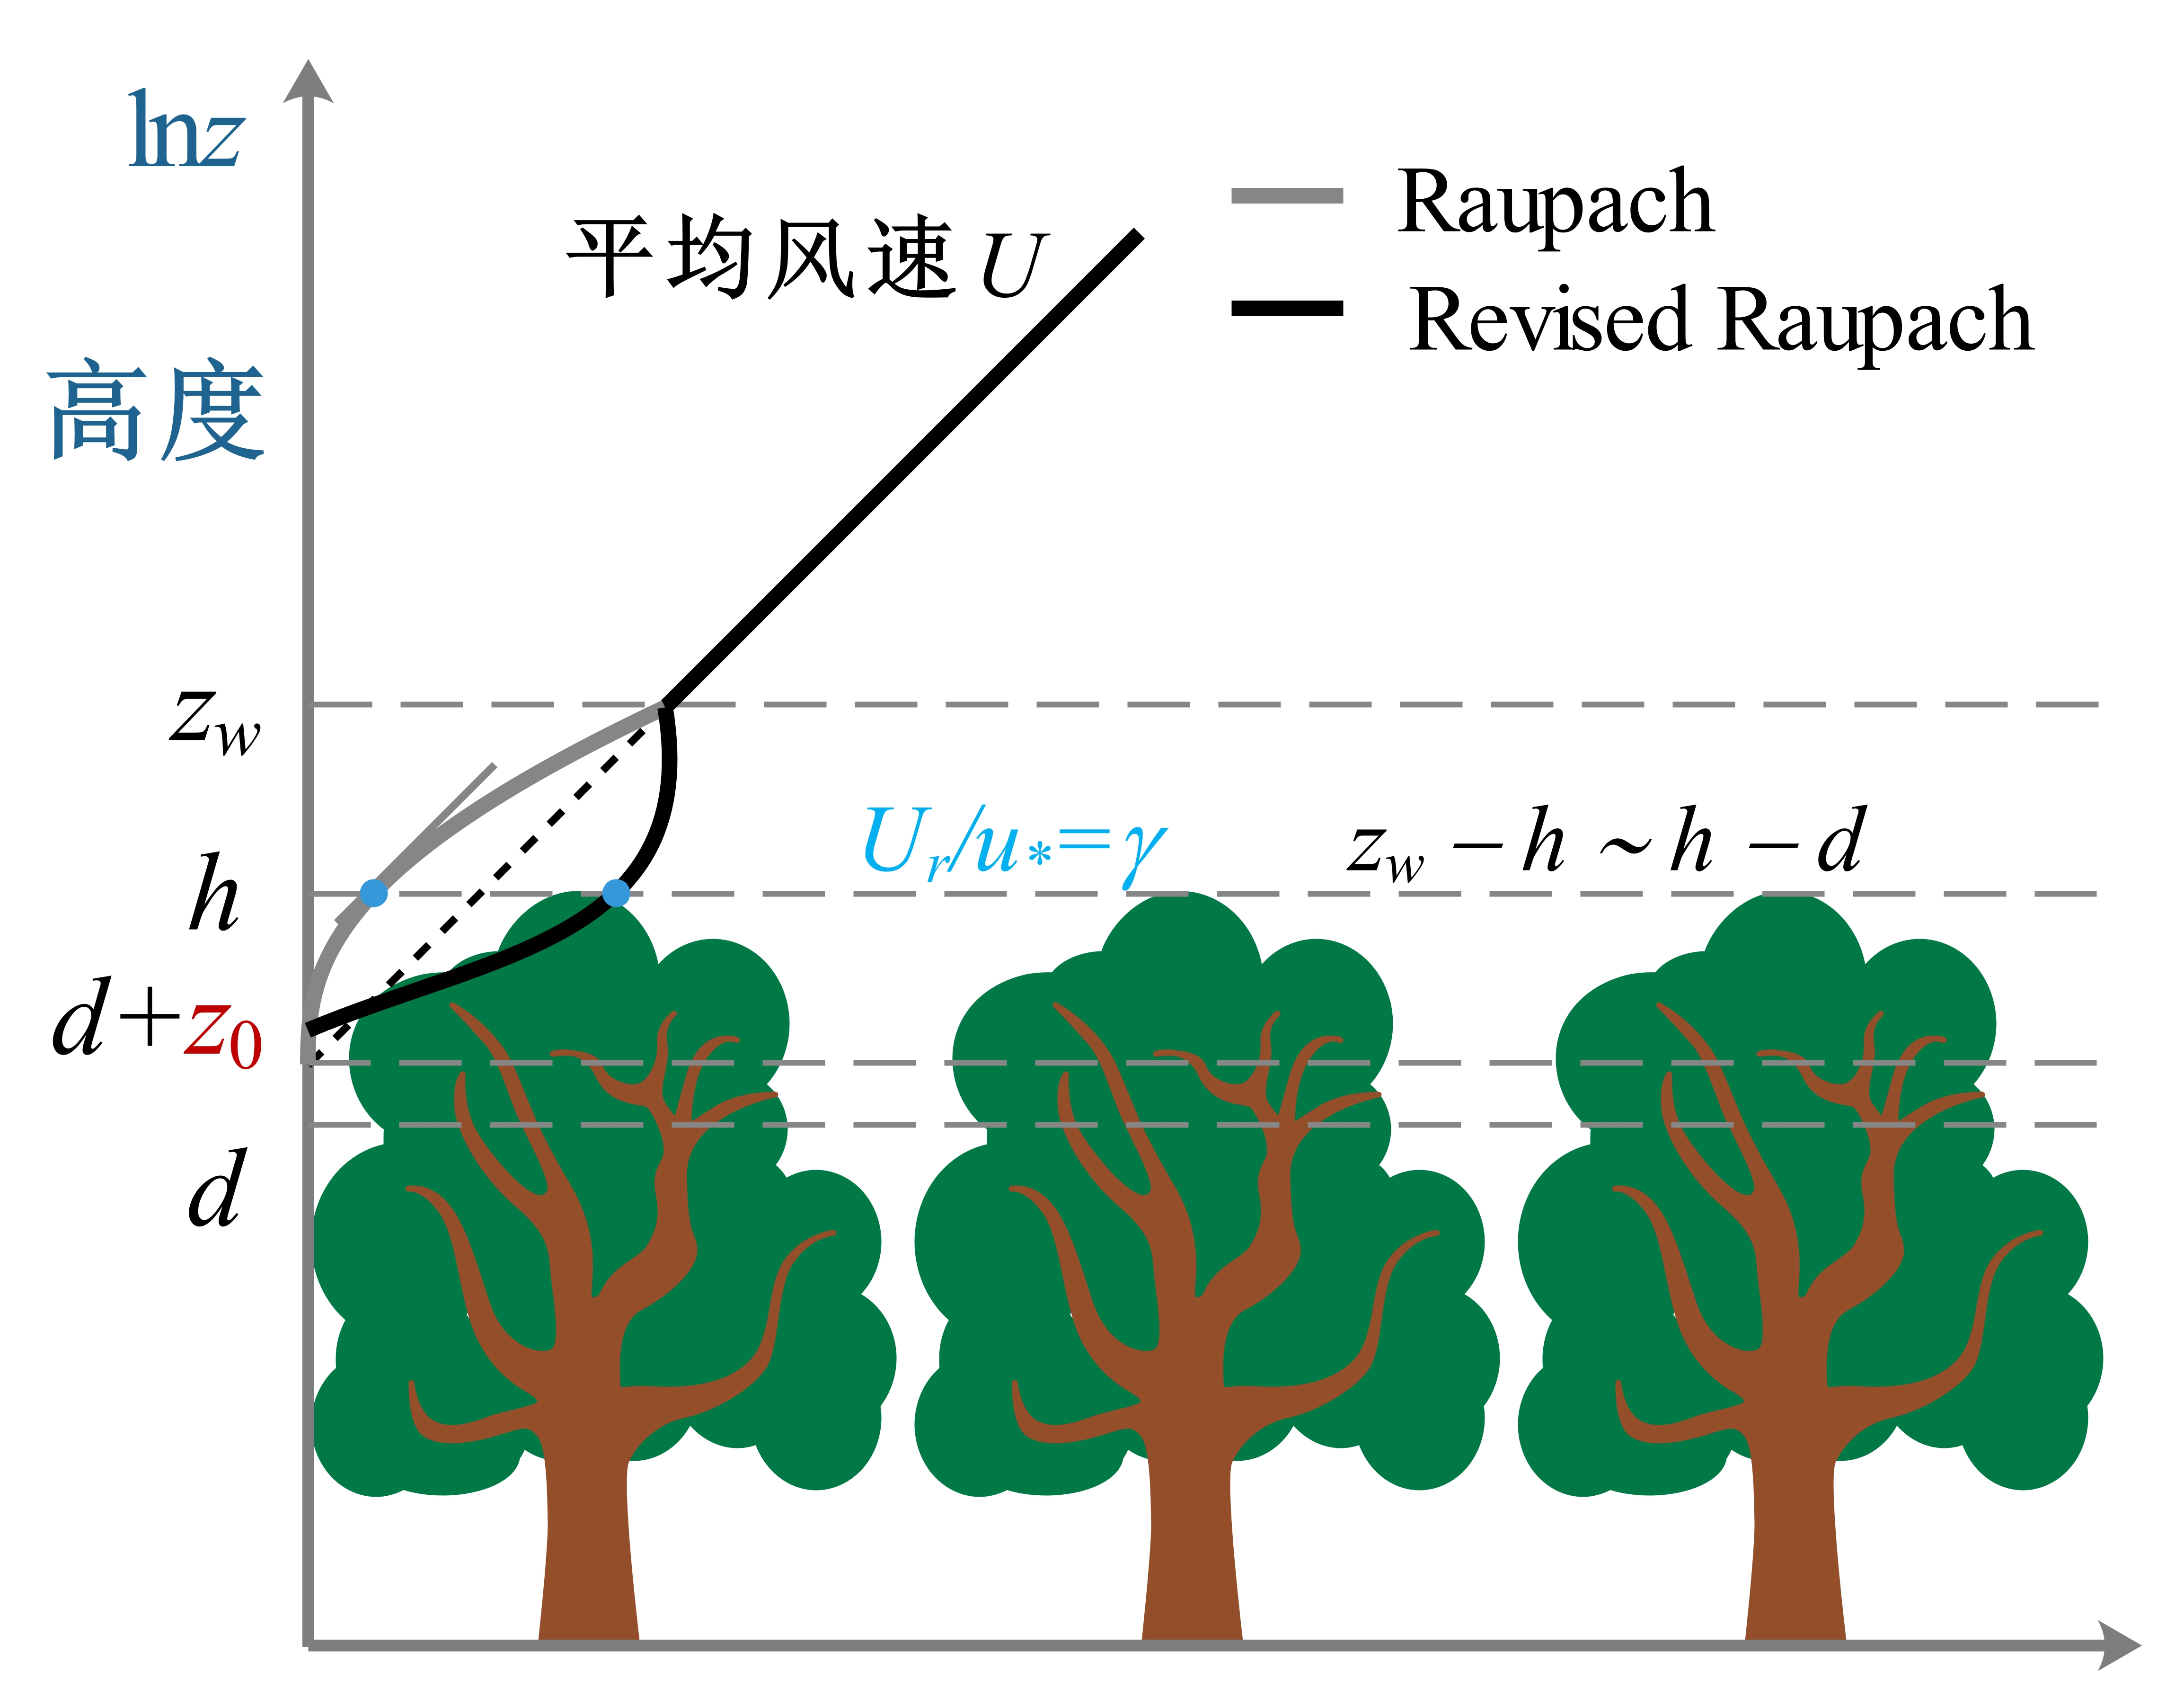
\includegraphics[scale=0.7]{Figures/地表湍流交换过程/修正Raupach粗糙度方案示意图.jpg}
\caption{考虑稳定度影响的植被粗糙度计算方案意图。}
\label{fig:修正Raupach粗糙度方案示意图}
\end{figure}
}


\subsection{单层植被湍流交换}
单层植被不同于100\%植被覆盖假设,而是考虑植被树冠之间可能存在空隙,
即植被树冠存在一定的水平分布,树冠覆盖度可介于0$\sim$100\%之间。这种植被结果假设与三维植被辐射模型假设一致。


对于植被树冠稀疏覆盖时,\citet{raupach1992drag,raupach1994simplified}通过场外和风洞实验,发展了一套用于计算$z_0$和$d$的解析解,其中:
\begin{equation}\label{dooh0}
\frac{d}{h}=1-\frac{1-\exp \left(-\sqrt{c_{d1} 2 \lambda}\right)}{\sqrt{c_{d1} 2 \lambda}}
\end{equation}
其中$c_{d1}=7.5$,$\lambda$%表示植被迎风面积指数 ($FAI$),
计算为$f_c\left(1-\exp{\left(-0.5LSAI\right)}\right)$。
当植被覆盖$f_c$等于100\%时,$\lambda$计算同100\%植被覆盖情景。为了同时适用与稀疏和浓密覆盖植被,
本版本采用\citet{dai2019different}方案计算$d$:
\begin{equation}\label{dooh}
\frac{d}{h}=f_{c} \cdot 1.1 \ln \left(1+\left(c_{d} f_{c} LAI\right)^{0.25}\right)+\left(1-f_{c}\right) \cdot\left(1-\frac{1-\exp \left(-\sqrt{c_{d1} 2 \lambda}\right)}{\sqrt{c_{d1} 2 \lambda}}\right)
\end{equation}
$z_0$的计算同公式 (\ref{zOh})。从上式可以看出,$d$值是100\%植被覆盖情景和稀疏植被按照植被覆盖度$f_c$的加权平均,
当$f_c\rightarrow100\%$时,公式 (\ref{dooh}) 趋同于公式 (\ref{dOh});当$f_c\rightarrow0\%$时,趋同于公式 (\ref{dooh0})。


对于植被冠层内的风速廓线$u$和湍流交换系数$K$,同样采用$f_c$加权方式。$u$和$K$分别计算为:
\begin{equation}
u(z)=f_{c} \cdot \min \left(u_{\exp }(z), u_{comb}(z)\right)+\left(1-f_{c}\right) \cdot u_{comb}
\end{equation}
\begin{equation}
\frac{1}{K(z)}=f_{c} \cdot \frac{1}{\min \left(K_{\exp}(z), K_{comb}(z)\right)}+\left(1-f_{c}\right) \cdot \frac{1}{K_{comb}}
\end{equation}
$u_{comb}$和$K_{comb}$同公式 (\ref{ucomb}) 和 (\ref{kcomb})。


\subsection{多层植被湍流交换}
多层植被湍流计算是以单层植被计算为基础,总体阻抗网络如图~\ref{fig:三层植被湍流交换示意图}所示。
风速$u$和湍流交换系数$K$廓线从最上层植被往下进行计算。上一层底部的廓线值作为下层植被顶部的值。
$r_b$和$r_d$的计算都是对$u$和$K$廓线的积分。
但积分区间对应到每层植被的等效交换高度(图~\ref{fig:三层植被湍流交换示意图} 中$T_{s1}$、$T_{s2}$、$T_{s3}$位置所示)。
该交换高度计算为该层植被100\%覆盖时的$d+z_0$值。在每一层等效交换高度,建议通量(感热H和潜热$\lambda E$)守恒方程,
即该点与上层通量交换量等于下层交换量加上该层植被的通量交换量。联立每层在等效高度建立的方程,迭代求解每种植被叶片温度。
{
\begin{figure}[]
\centering
\includegraphics{Figures/地表湍流交换过程/三层植被湍流交换示意图.png}
\caption{三层植被湍流交换示意图。}
\label{fig:三层植被湍流交换示意图}
\end{figure}
}


通过以上介绍可以看出,三维植被湍流交换与一维植被湍流交换最大的不同在于其计算的对象由原来单一植被扩展到多个分层植被,
阻抗网络发生变化,多种植被在同一环境下同时求解。在计算时,同一维植被一样,需要用到植被短波辐射吸收量和长波辐射吸收量,
此时利用章节~\ref{三维植被辐射传输模型} 和 \ref{三维植被长波辐射传输} 对三维植被辐射传输计算结果。整个植被冠层与大气的湍流交换同样采用相似性理论进行求解,
其求解过程如图~\ref{fig:三维植被湍流交换模型计算流程图} 所示。
{
\begin{figure}[]
\centering
\includegraphics{Figures/地表湍流交换过程/三维植被湍流交换模型计算流程图.png}
\caption{三维植被湍流交换模型计算流程图。}
\label{fig:三维植被湍流交换模型计算流程图}
\end{figure}
}
